\documentclass[addpoints]{exam}

    \makeatletter % Lagfæring fyrir nýjar útgáfur af TeXLive
    \expandafter\providecommand\expandafter*\csname ver@framed.sty\endcsname
    {2003/07/21 v0.8a Simulated by exam}
    \makeatother
    
    \usepackage[top=2cm, bottom=2cm, left=1cm, right=1cm]{geometry}
    \usepackage[utf8]{inputenc}
    \usepackage[icelandic]{babel}
    \usepackage[T1]{fontenc}
    % \usepackage[sc]{mathpazo}
    \usepackage{helvet} \renewcommand\familydefault{\sfdefault}
    
    \usepackage[parfill]{parskip}
    \usepackage{tabularx, booktabs}
    \usepackage{multirow}
    \usepackage{multicol}
    \usepackage{graphicx, tikz}
    \usepackage{enumerate}
    \usepackage{amsmath, amsfonts, amssymb, amsthm}
    \usepackage{minted} %Minted and configuration
    \usepackage{afterpage}
    \usepackage{scrextend}
    
    \usepackage[pdftex,bookmarks=true,colorlinks=true,pdfauthor={Eirikur Ernir Thorsteinsson},linkcolor=blue,urlcolor=blue]{hyperref}
    
    \newmintedfile[cppfile]{cpp}{frame=lines, linenos=false}
    \newmintedfile[javafile]{java}{frame=lines, linenos=false}
    \newcommand{\eng}[1]{(e.\ \emph{#1})}

    \setcounter{secnumdepth}{-1} 
    \hyphenpenalty=5000
    
    \newcommand\blankpage{%
        \null
        \thispagestyle{empty}%
        \addtocounter{page}{-1}%
        }
    
    \usemintedstyle{default}
    \renewcommand{\theFancyVerbLine}{\sffamily \arabic{FancyVerbLine}}
    \author{}
    \date{}
    
    \footer{}{}{}
    
    \setcounter{secnumdepth}{-1} 
    
    \qformat{\large \textbf Spurning \thequestion \phantom{M}(\totalpoints \phantom{l}stig) \hfill}
    \renewcommand{\solutiontitle}{\noindent\textbf{Svar:}\par\noindent}
    \renewcommand{\points}{stig}
    \renewcommand{\questionshook}{\setlength{\itemsep}{0.5cm}}
    \hqword{Spurning:}
    \hpword{Stig í boði:}
    \hsword{Stig:}
    \htword{Samtals}
    
    \title{TÖL203G Tölvunarfræði 2 - lokapróf}
    \author{}
    \date{maí 2018}
    
    \pagestyle{headandfoot}
    \firstpageheader{TÖL203G}{Tölvunarfræði 2 - Lokapróf}{maí 2018}
    \firstpagefooter{}{Bls. \thepage\ af \numpages}{}
    \runningfooter{}{Bls. \thepage\ af \numpages}{}
    \setlength{\columnsep}{0.5cm}
    
    \changefontsizes{14pt}

\begin{document}

Fullt nafn: \vspace*{1mm} \hrule

\vspace{1cm}

\textbf{Leiðbeiningar:} Á þessu prófi eru \numquestions\ spurningar sem samtals gefa \numpoints\ stig.
Leyfileg hjálpargögn eru reiknivél og ein A4 blaðsíða af glósum.

Heftið verður skannað inn í tölvu til yfirferðar. Vinsamlegast forðist ljósa blýanta, ekki rífa eða krumpa heftið og ekki bæta við blaðsíðum eða fjarlægja.

Til að svara krossaspurningum skal nota svartöfluna hér að neðan. Merkið vandlega við einn möguleika fyrir hverja spurningu. Ekki er dregið frá fyrir röng svör. 

Til að svara öðrum spurningum skal skrifa inn í svæðið sem fylgir strax á eftir hverri spurningu. Þurfi að koma viðbótarupplýsingum til skila skal skrifa það í rammana á
öftustu blaðsíðunum. Aðrir hlutar heftisins, sér í lagi bakhliðar, verða ekki lesnir.

Dæmin á þessu prófi eru misþung. Þau eru ekki sett fram í erfiðleikaröð.

\begin{center}
	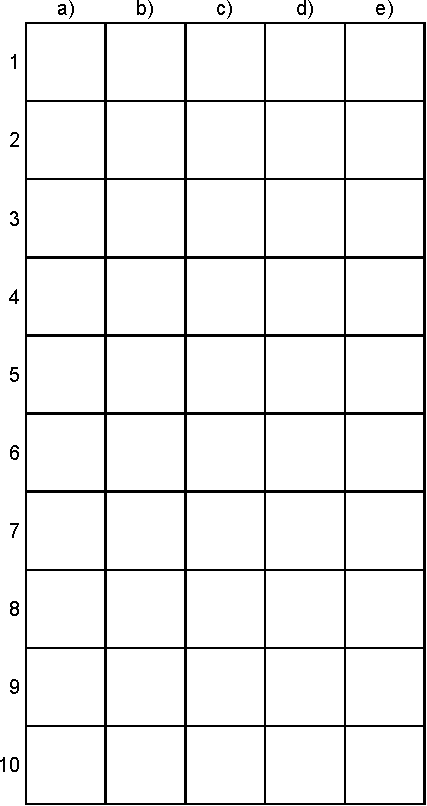
\includegraphics[width=0.4\linewidth]{Pics/svartafla}
\end{center}

\newpage

\begin{questions}

	\section{Krossaspurningar}

	\question[3]

	Hvert af eftirfarandi er ekki hugræn gagnagerð \eng{abstract data type}?

	\begin{enumerate}[a)]
		\item Skjóða
		\item Hlaði
		\item Biðröð
		\item Eintengdur listi
		\item Net
	\end{enumerate}

	\question[3]

	Þegar breytan \texttt{i} er búin til innan falls í C++ með skipuninni \texttt{int i = 0;} er líftími hennar að óbreyttu\ldots

	\begin{enumerate}[a)]
		\item Frumstæður \eng{primitive}
		\item Kyrrstæður \eng{static}
		\item Kvikstæður \eng{dynamic}
		\item Sérstæður \eng{particular}
		\item Sjálfvirkur \eng{automatic}
	\end{enumerate}

	\question[3]

	Gefið er eftirfarandi C++ fall. Hvert er vandamálið við það?

	\begin{minted}[frame=lines]{cpp}
int* f( int a ) {
  int b = 2*a;
  return &b;
}
    \end{minted}

	\begin{enumerate}[a)]
		\item Fallið er málfræðilega rangt
		\item Fallið skilar ekki bendi á heiltölu
		\item Fallið tekur ekki frá minni fyrir breytuna \texttt{b}
		\item Fallið skilar alltaf \texttt{nullptr}
		\item Fallið skilar minnissvæði af hlaðanum
	\end{enumerate}

	\newpage

	\question[3]

	Gefið er C++ forrit.

	\cppfile[firstline=4, fontsize=\small, linenos=true]{Code/w14/Animals.cpp}

	Hvaða áhrif myndi það hafa að bæta orðinu \texttt{virtual} fremst í línu 6, svo þar stæði \texttt{virtual void move()}?

	\begin{enumerate}[a)]
		\item Forritið myndi skrifa út ``Dog runs!'' í stað ``Animal moves!''
		\item Forritið myndi skrifa út ``Animal moves!'' í stað ``Dog runs!''
		\item Engin áhrif, forritið myndi áfram skrifa út ``Animal moves!''
		\item Engin áhrif, forritið myndi áfram skrifa út ``Dog runs!''
		\item Forritið myndi ekki þýðast
	\end{enumerate}

	\question[3]

	Sé biðröð \eng{queue} útfærð á skynsamlegan hátt með eintengdum lista, af hvaða stærðargráðu er tími innsetningar og eyðingar?

	\begin{enumerate}[a)]
		\item  $1$ (fasti) innsetning og eyðing
		\item  $\log N$ innsetning og eyðing
		\item  $1$ innsetning, $N$ eyðing
		\item  $N$ innsetning, $1$ eyðing
		\item  $N$ innsetning og eyðing
	\end{enumerate}

	\question[3]
	Af hvaða stærðargráðu er keyrslutími sameiningarröðunar \eng{merge sort} á $N$ staka fylki?

	\begin{multicols}{5}
		\begin{enumerate}[a)]
			\item $1$ (fasti)
			\item $\log N$
			\item $N$
			\item $N\log N$
			\item $N^2$
		\end{enumerate}
	\end{multicols}

	\question[3]
	$N$ lyklar eru settir inn í \emph{lækkandi} röð í nafnatöflu \eng{symbol table} sem útfærð er með einföldu tvíleitartré. Af hvaða stærðargráðu verður keyrslutími einnar uppflettingar í nafnatöflunni?

	\begin{multicols}{5}
		\begin{enumerate}[a)]
			\item $1$ (fasti)
			\item $\log N$
			\item $N$
			\item $N\log N$
			\item $N^2$
		\end{enumerate}
	\end{multicols}

	\question[3]
	$N$ lyklar eru settir inn í \emph{lækkandi} röð í max-forgangsbiðröð sem útfærð er með hrúgu. Af hvaða stærðargráðu er heildarinnsetningartíminn?

	\begin{multicols}{5}
		\begin{enumerate}[a)]
			\item $1$ (fasti)
			\item $\log N$
			\item $N$
			\item $N\log N$
			\item $N^2$
		\end{enumerate}
	\end{multicols}

	\question[3]

	Hvert af eftirfarandi er vandamál við að nota grennslafylki til að útfæra klasa sem táknar net?

	\begin{enumerate}[a)]
		\item Útfærslan er mun flóknari en útfærsla með grennslalistum
		\item Erfitt er að sjá út frá grennslafylki hvort að tveir hnútar séu aðlægir
		\item Minnisnotkunin vex með hnútafjölda í öðru veldi
		\item Minnisnotkunin vex með leggjafjölda í öðru veldi
		\item Fylki henta skyndiminni örgjörva verr en listar
	\end{enumerate}

	\question[3]

	Hvert eftirfarandi reiknirita má nota til að finna stystu leið á milli tveggja hnúta í neti sem ekki er vegið?

	\begin{enumerate}[a)]
		\item Reiknirit Prims
		\item Reiknirit Kruskals
		\item Dýptarleit
		\item Breiddarleit
		\item Reiknirit Sierpinskis
	\end{enumerate}

	\section{Skrifleg verkefni}

	\question[5]
	Listar og fylki gegna svipuðu hlutverki í forritun - að geyma stök sem aðgengileg eru eftir númerum. Nefnið einn kost og einn galla við að geyma gögn í eintengdum lista í stað þess að nota fylki.

	\makeemptybox{\stretch{1}}

	\question[5]
	Quicksort-útfærsla Sedgewicks og Wayne slembiraðar safninu áður en hið eiginlega reiknirit hefst. Nefnið einn kost og einn galla við þetta fyrirkomulag.

	\makeemptybox{\stretch{1}}

	\newpage

	\question[5]

	Eftirfarandi tafla lýsir hakkafalli á enska stafrófið:

	\begin{center}
		\scriptsize
		\begin{tabular}{l*{26}{c}}
			\toprule
			$x$    & A & B & C & D & E & F & G & H & I & J & K & L & M & N & O & P & Q & R & S & T & U & V & W & X & Y & Z \\
			\midrule
			$f(x)$ & 5 & 0 & 4 & 0 & 5 & 2 & 3 & 3 & 4 & 3 & 1 & 0 & 0 & 1 & 3 & 0 & 5 & 2 & 3 & 3 & 2 & 3 & 5 & 5 & 4 & 0 \\
			\bottomrule
		\end{tabular}
	\end{center}

	Teiknið ``separate chaining'' hakkatöflu sem notar þetta hakkafall. Sýnið ástandið eftir að að lyklarnir T O L V U N A R F R A E D I eru settir inn í hana í röð, væri taflan tóm í upphafi. Látið gildin vera númer lykilsins (í innsetningarröð, fyrsta talan 0).

	\makeemptybox{\stretch{1}}

	%	\question[5]

	%	Lýsið því hvernig árekstrar eru útkljáðir í “linear probing” hakkatöflu.

	%	\makeemptybox{\stretch{1}}

	\newpage

	\section{Forritunarspurningar}

	\question[10]

	Skrifið Java-aðferðina \texttt{removeOdds} sem tekur inn hlaða (\texttt{Stack}) heiltalna og fjarlægir úr honum allar oddatölur, en breytir honum ekki að öðru leyti.

	Haus aðferðar: \texttt{void removeOdds(Stack<Integer> s)}

	\makeemptybox{\stretch{1}}

	\newpage

	\question[10]

	Skrifið C++ aðferðina \texttt{remove} sem fjarlægir hnút númer \texttt{i} úr eintengdum lista. Ef \texttt{i} er 0 þá er fremsti hnúturinn fjarlægður, ef \texttt{i} er 1 þá er næstifremsti hnúturinn fjarlægður, o.s.frv. Klasauppbyggingu má sjá í viðauka. 
	
	Gera má ráð fyrir að \texttt{0 <= i <= length - 1} þegar aðferðin er notuð.

	Haus aðferðar: \texttt{void remove(int i)}

	\makeemptybox{\stretch{1}}

	\newpage

	\question[10]

	Skrifið helmingunarleit í Java. Aðferðin skal taka inn fylki af stígandi heiltölum ásamt heiltölu sem leita skal að. Hún skal skila sætisnúmeri í fylkinu þar sem leitarstakið er að finna. Sé leitarstakið ekki í fylkinu skal aðferðin skila tölunni -1.

	Haus aðferðar: \texttt{int binarySearch(int[] a, int key)}

	\makeemptybox{\stretch{1}}

	\newpage

	\question[10]

	Gefinn er hluti af útfærslu á rauðsvörtu tré í viðauka. Skrifið Java-aðferð sem tekur inn hnút og athugar hvort tréð sem hefur þann hnút sem rót sé löglegt rauðsvart tré með tilliti til reglna um rauðar og svartar tengingar.

	Haus aðferðar: \texttt{boolean isRedBlackTree(Node node)}

	\makeemptybox{\stretch{1}}

	\paragraph{Ath:} Ekki þarf að athuga hvort tréð sé löglegt tvíleitartré að öðru leyti.

	\newpage

	%	\question[10]

	%	Stefnd net án örvarása hafa þann eiginleika að fyrir þau má finna röðun \eng{topological ordering} svo að allir leggir netsins vísi í sömu átt. Sjá mynd í viðauka. Skrifið Java-aðferðina \texttt{ordering} sem tekur inn stefnt net (\texttt{Digraph}) og skilar slíkri röðun sem runu af hnútanúmerum (t.d. fylki eða \texttt{Iterable} hlut).

	%	\paragraph{Ábending:} Hægt er að nota aðferð sem líkist dýptarleit.

	\question

	\begin{parts}

		\part[5]

        Skrifið Java-aðferðina \texttt{merge} sem tekur inn tvær biðraðir (\texttt{Queue}) sem innihalda stök í stígandi röð og skilar biðröð sem inniheldur stök beggja biðraðanna í stígandi röð.
        
        Haus aðferðar: \texttt{static <Item extends Comparable<Item> > \\ Queue<Item> merge(Queue<Item> q1, Queue<Item> q2)}

        \makeemptybox{\stretch{1}}
        
        \newpage

		\part[10]

        Skrifið útgáfu af ``bottom-up'' sameiningarröðun sem byggist á biðröðum. Skiptið $N$ staka safninu niður í $N$ biðraðir sem hver inniheldur eitt stak. Notið svo sameiningaraðferðina úr a)-lið endurtekið þar til eingöngu ein biðröð er eftir.

        Haus aðferðar: \texttt{void sort(Comparable[] a)}.
        
        \makeemptybox{\stretch{1}}

        \paragraph{Ath:} Í þessu dæmi má gera ráð fyrir að a)-liðurinn hafi verið rétt útfærður.

	\end{parts}


\end{questions}

\newpage

\section{Viðbótarpláss}

Eftirfarandi viðbótarpláss verður skannað inn. Sé það notað, vísið til þess í viðkomandi spurningu.

\makeemptybox{\stretch{1}}

\newpage

\makeemptybox{\stretch{1}}

\newpage

\section{Viðauki}
Eftirfarandi skil úr \emph{Algorithms, 4th edition} eru gefin:
\begin{center}
	%	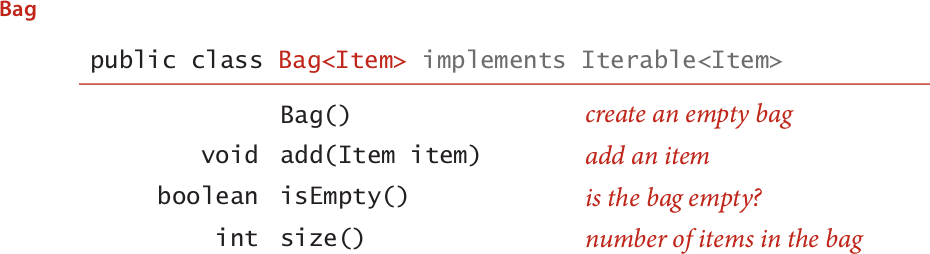
\includegraphics[width=0.8\textwidth]{Pics/API-Bag}

	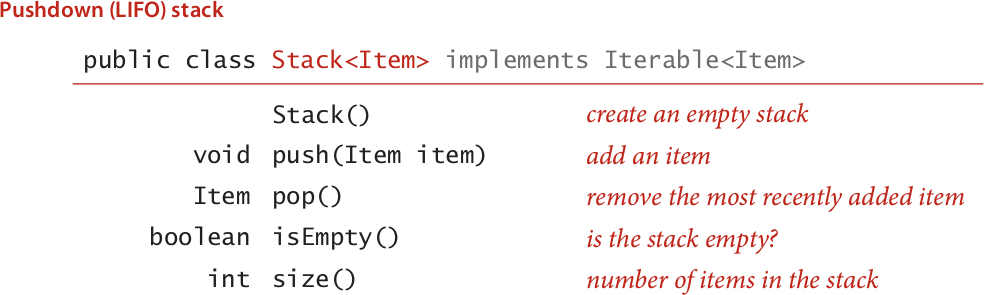
\includegraphics[width=0.7\textwidth]{Pics/API-Stack}

	\vspace{0.5cm}

	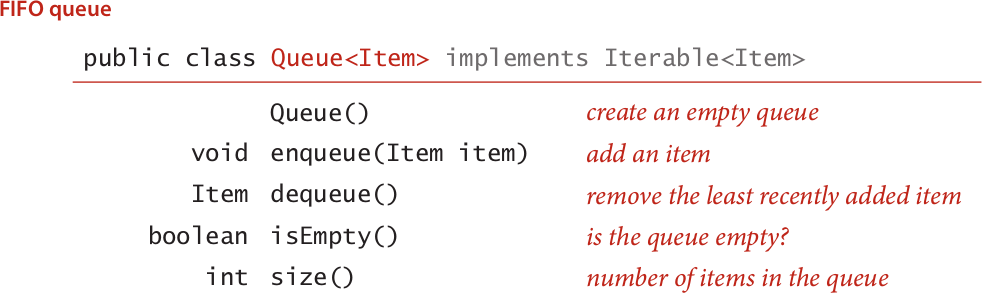
\includegraphics[width=0.7\textwidth]{Pics/API-Queue}

	%	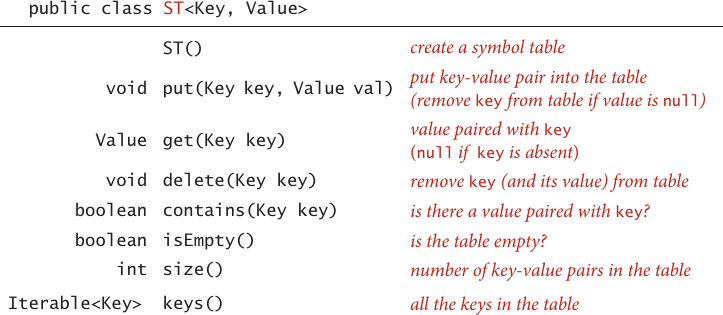
\includegraphics[width=0.8\textwidth]{Pics/API-ST}

	%	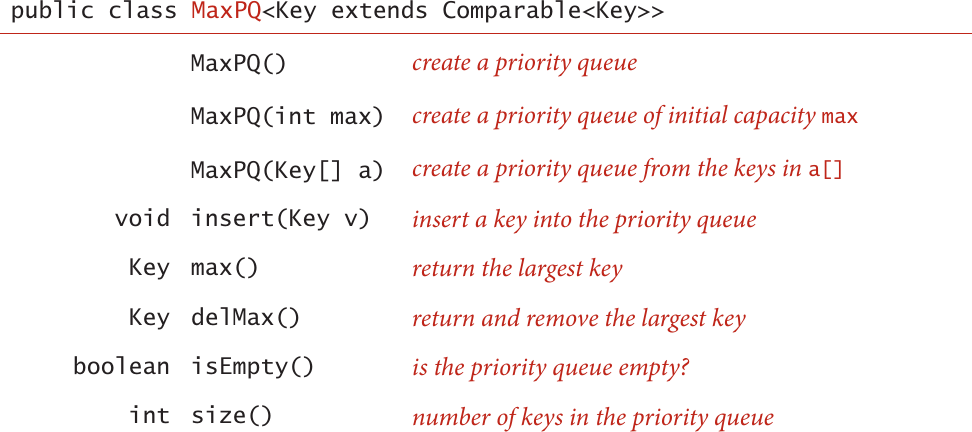
\includegraphics[width=0.8\textwidth]{Pics/API-MaxPQ}

	%	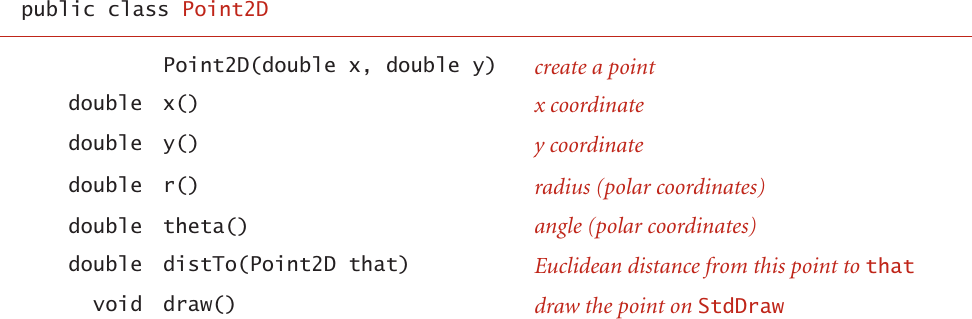
\includegraphics[width=0.8\textwidth]{Pics/API-Point2d}

	%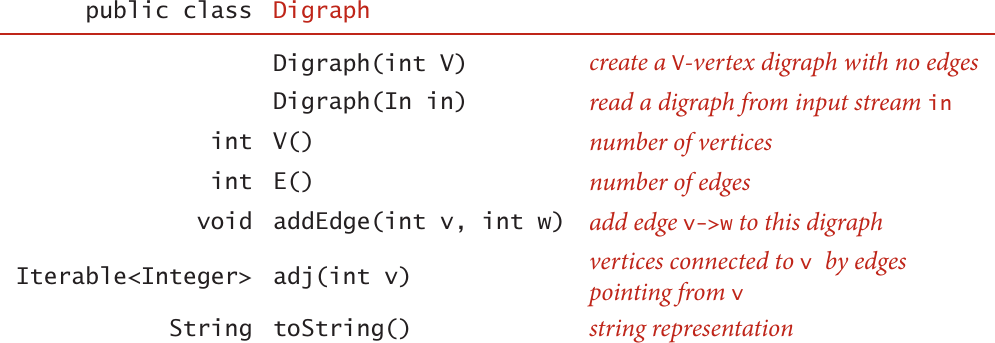
\includegraphics[width=0.8\textwidth]{Pics/API-Digraph}

	% 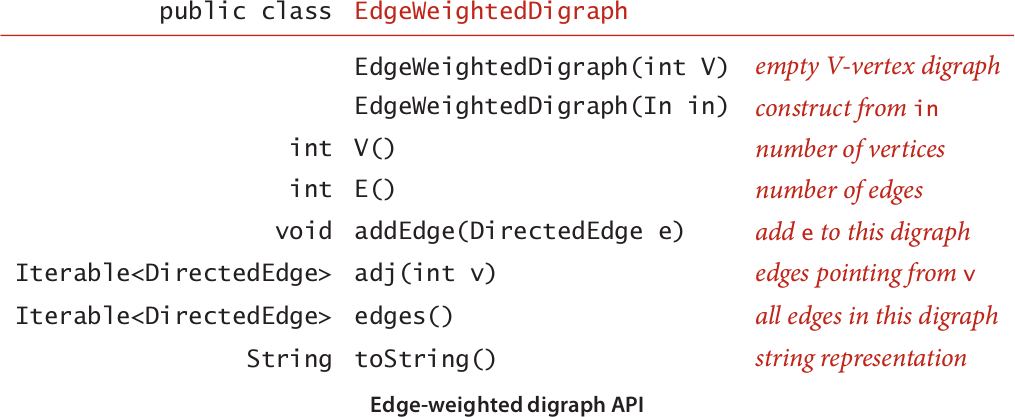
\includegraphics[width=0.8\textwidth]{Pics/API-EWDG}

	% \vspace{1cm}

	% 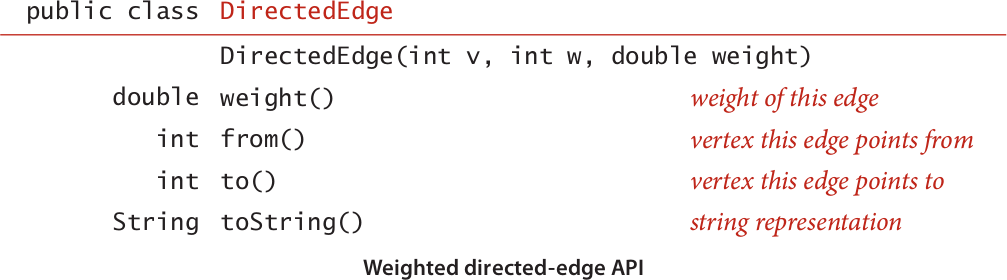
\includegraphics[width=0.8\textwidth]{Pics/API-DE}

	% \vspace{1cm}

    % 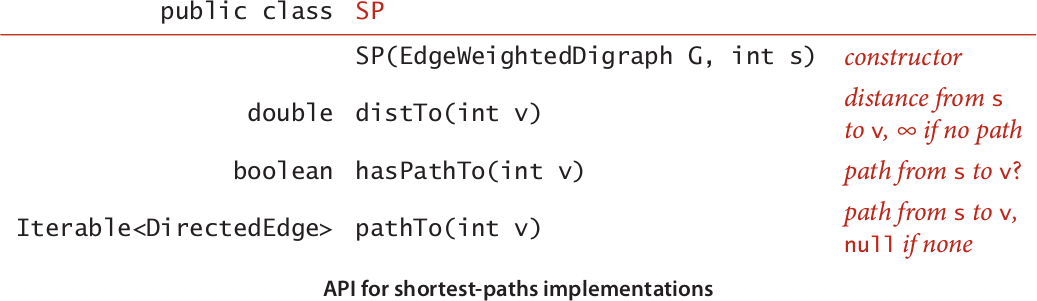
\includegraphics[width=0.8\textwidth]{Pics/API-SP}
    
\end{center}

	Klasar fyrir dæmi 15 og 17.
	\begin{multicols}{2}
		\cppfile[fontsize= \scriptsize]{Code/w14/LinkedList.cpp}

        \vspace{1cm}

		\javafile[fontsize= \scriptsize]{Code/w14/RedBlackTree.java}
	\end{multicols}

%%	Til vinstri: Stefnt rásalaust net. Til hægri: Röðunin 2 0 1 4 3 á netinu.
%%
%	\usetikzlibrary{arrows}
%	\begin{tikzpicture}
%		\tikzset{edge/.style = {->,> = latex'}}
%		\node (c1) at (2, 3) {2};
%		\node (d1) at (3, 2) {0};
%		\node (e1) at (3, 4) {1};
%		\node (f1) at (0, 3) {4};
%		\node (g1) at (0, 1) {3};
%
%		\draw[edge] (c1) to (f1);
%		\draw[edge] (c1) to (g1);
%		\draw[edge] (d1) to (e1);
%		\draw[edge] (e1) to (f1);
%
%		\node (c2) at (6, 1) {2};
%		\node (d2) at (6, 2) {0};
%		\node (e2) at (6, 3) {1};
%		\node (f2) at (6, 4) {4};
%		\node (g2) at (6, 5) {3};
%
%		\draw[edge] (c2) to[bend right=70] (f2);
%		\draw[edge] (c2) to[bend left=70] (g2);
%		\draw[edge] (d2) to (e2);
%		\draw[edge] (e2) to (f2);
%	\end{tikzpicture}

\end{document}